\documentclass{beamer}
\mode<presentation>
\usetheme{sidebar}
\setbeamertemplate{footline}[page number]

\title{Kentekenherkenning met Local Binary Patterns}
\date{23 december 2011}
\author{
    Gijs van der Voort\\
    Fabi\"en Tesselaar\\
    Richard Torenvliet\\
    Tadde\"us Kroes\\
    Jayke Meijer
}

\begin{document}

    \begin{frame}
        \titlepage
    \end{frame}

    \section{Inleiding}

    \begin{frame}
        \frametitle{Probleemomschrijving}

        \begin{itemize}
            \item Herkennen van kentekens met LBP
            \item Focus op herkennen enkele karakters
        \end{itemize}
    \end{frame}

    \begin{frame}
        \frametitle{Doel}

        \begin{enumerate}
            \item Omzetten van dataset naar afzonderlijke karakters
            \item Karakter normaliseren
            \item Feature vector maken met LBP
            \item SVM classifier trainen met feature vectors
            \item Meten van performance
        \end{enumerate}
    \end{frame}

    \section{Local Binary Patterns}

    \begin{frame}
        \frametitle{Wat is een Local Binary Pattern?}

        \begin{itemize}
            \item Vergelijken van grijswaardes op lokaal niveau
            \item Ongevoelig voor verschillen in belichting (gray-scale
            invariant)
            \item Simpel algoritme, dus snelle implementatie mogelijk
        \end{itemize}
    \end{frame}

    \section{Implementatie}

    \begin{frame}
        \frametitle{Omzetten karakters}

        \begin{itemize}
            \item Dataset bestaat uit foto's van kentekens met informatie over
            locaties van karakters
            \item Dataset bevat veel fouten
            \item Eenmalige operatie
        \end{itemize}
    \end{frame}

    \begin{frame}
        \frametitle{Karakter normaliseren}

        \begin{itemize}
            \item Transformeer alle karakters naar dezelfde hoogte om dikte te
            normaliseren
            \item Ruisonderdrukking m.b.v. Gaussian blur
        \end{itemize}
    \end{frame}

    \begin{frame}
        \frametitle{Feature vector maken met LBP}

        \begin{enumerate}
            \item Kies een pixel
            \pause
            \item Kies een aantal buren van de pixel
            \begin{figure}
                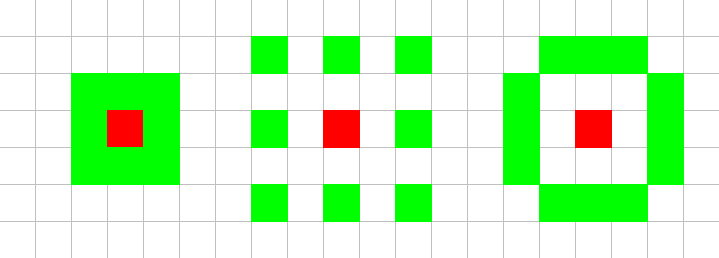
\includegraphics[scale=.3]{neighbourhoods.png}
            \end{figure}
            \pause
            \item Vergelijk de grijswaarde van de eerder gekozen pixel met de
            grijswaarde van zijn buren, elke vergelijking levert een 1 of 0 op
            \pause
            \item Deze binaire waardes samen vormen \'e\'en LBP
            \pause
            \item Maak een histogram van elke cel in de afbeelding,
            concatenatie van histogrammen is de feature vector
        \end{enumerate}
    \end{frame}

    \begin{frame}
        \frametitle{Trainen SVM classifier}

        \begin{itemize}
            \item Radial kernel function
            \item Gebruik \texttt{libsvm}
        \end{itemize}
    \end{frame}

    \section{Resultaten}

    \begin{frame}
        \frametitle{Parameter Gaussian blur: $\sigma$}

        \begin{itemize}
            \item Theorie: proportioneel aan de dikte van een letter
            \item Beste resultaat met $\sigma = 1.9$ \\
            $1.9 \cdot 6 = 11$ pixels, breedte karakter is 8 pixels
        \end{itemize}
    \end{frame}

    \begin{frame}
        \frametitle{Parameters SVM: Soft-margin en $\gamma$}

        \begin{itemize}
            \item Bepaald door grid-search:
            \begin{itemize}
                \item Kies exponentieel oplopende waardes voor $C$ en $\gamma$
                \item Train een SVM voor elke combinatie van waardes
                \item Zet de resultaten in een tabel
            \end{itemize}
            \item Beste resultaat met $C = 32.0$ en $\gamma = 0.125$
        \end{itemize}
    \end{frame}

    \begin{frame}
        \frametitle{Meten van performance}

        \begin{itemize}
            \item Accuratie
            \begin{itemize}
                \item Score van $94.3\%$
            \end{itemize}
            \item snelheid bij standaardhoogte van 42 pixels:
            \begin{itemize}
                \item $3 \times 3$ omgeving (8 pixels in patroon): 81ms
                \item $5 \times 5$ omgeving (12 pixels in patroon): 137ms
                \item feature vector $16\times$ groter, $1.7\times$ zoveel tijd
            \end{itemize}
        \end{itemize}
    \end{frame}

    \begin{frame}
        \frametitle{Foutief geclassificeerde karakters}

        \begin{figure}
            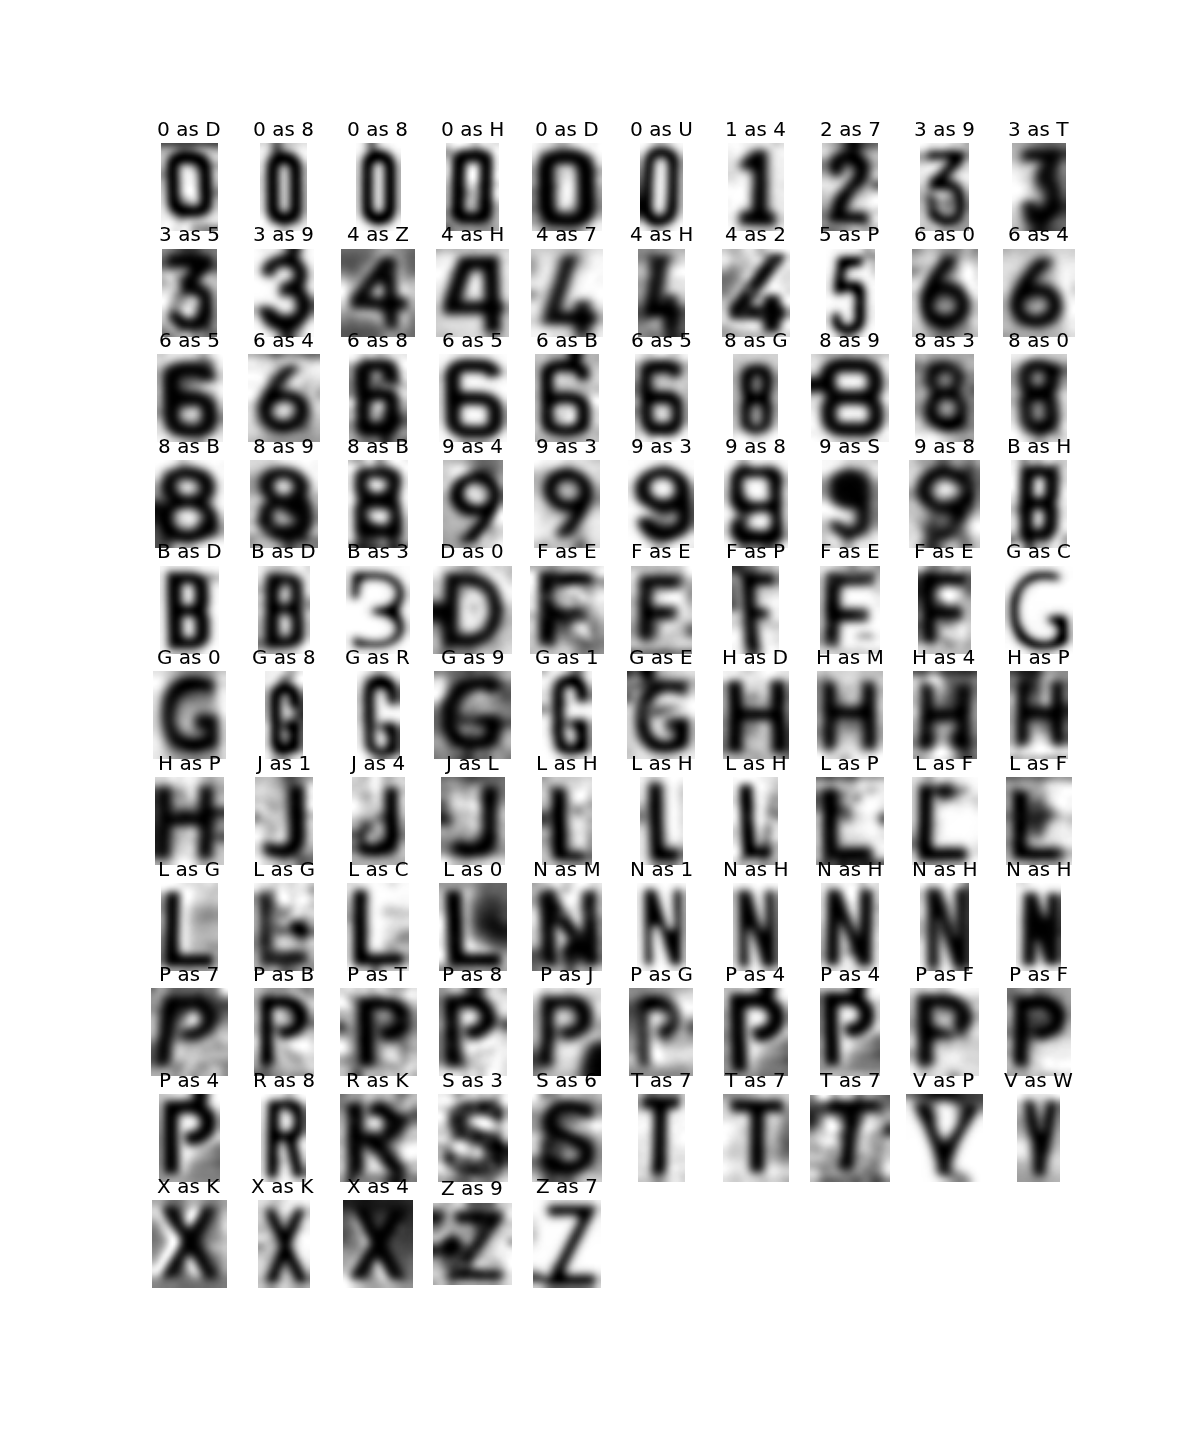
\includegraphics[scale=.2]{faulty.png}
        \end{figure}
    \end{frame}

    \section{Mogelijkheden voor vervolgonderzoek}

    \begin{frame}
        \frametitle{Mogelijkheden voor vervolgonderzoek}

        \structure{Accuratie}
        \begin{itemize}
            \item Meerdere cells
            \item Andere pixelpatronen voor LBP
            \item Betere verdeling leerset/testset
            \item Toevoegen contextinformatie
        \end{itemize}

        \structure{Snelheid}
        \begin{itemize}
            \item Rekenintentensieve taken vertalen naar C
            \item Andere kernel type
            \item `Cachen' Gaussian filter
        \end{itemize}
    \end{frame}

    \section{Conclusie}

    \begin{frame}
        \frametitle{Conclusie}

        \begin{itemize}
            \item LBP is een geschikt algoritme voor gebruik in
            kentekenherkenning
            \item Zowel accuratie als snelheid
        \end{itemize}
    \end{frame}

    \section{Referenties}

    \begin{frame}
        \frametitle{Referenties}

        \begin{itemize}
            \item \url{http://en.wikipedia.org/wiki/Local\_binary\_patterns}
            \item \url{http://en.wikipedia.org/wiki/Support\_vector\_machine}
            \item \url{http://www.csie.ntu.edu.tw/~cjlin/libsvm/}
        \end{itemize}
    \end{frame}
\end{document}
